\documentclass{article}
\usepackage[utf8]{inputenc}
\usepackage[a4paper, left=3cm, right=3cm, top=2.5cm, bottom=2.5cm]{geometry}
\renewcommand{\thesection}{\Roman{section}.}
\renewcommand{\thesubsection}{\Alph{subsection}.}
\renewcommand{\thesubsubsection}{\alph{subsubsection}.}
\usepackage{amsmath}        % For \text{}, align, equation
\usepackage{amssymb}        % For \mathbb{}
\usepackage{amsfonts}       % For math fonts
\usepackage{algorithm}      % For algorithm environment
\usepackage{algorithmic}    % For algorithmic environment
\usepackage{listings}       % For lstlisting (code)
\usepackage{bm}            % For \boldsymbol
\usepackage{graphicx}
\usepackage{parskip} % Automatically sets \parindent=0pt and \parskip to a nice value
\usepackage{fancyhdr}
\usepackage{indentfirst}
\usepackage{caption}
\captionsetup{font=footnotesize}  % This sets caption to 9pt

% \pagestyle{fancy}
\fancyhf{}
\cfoot{\thepage}
\setlength{\parindent}{0.5cm}  
\title{Progress \textit{Automatic Modulation Classification} Menggunakan CNN+LSTM Standart (Serial) dan Parallel}
% \author{Muhammad Alif Fadhilah (NIU : 552180)}
\date{\today}

\begin{document}

\maketitle
\section{Konfigurasi Dataset}

\subsection{Skema Modulasi Target}
Sistem dirancang untuk mengklasifikasikan \textbf{9 jenis modulasi digital} yang berbeda. Setiap jenis modulasi memiliki karakteristik unik dalam representasi sinyal I/Q yang memungkinkan model untuk membedakan antara satu jenis dengan jenis lainnya.

\begin{table}[h]
\centering
\caption{Daftar Skema Modulasi Target}
\label{tab:target_modulations}
\begin{tabular}{|c|l|l|}
\hline
\textbf{Indeks Kelas} & \textbf{Modulasi} & \textbf{Deskripsi} \\
\hline
0 & OOK & On-Off Keying \\
1 & 4ASK & 4-ary Amplitude Shift Keying \\
2 & 8ASK & 8-ary Amplitude Shift Keying \\
3 & BPSK & Binary Phase Shift Keying \\
4 & QPSK & Quadrature Phase Shift Keying \\
5 & 8PSK & 8-ary Phase Shift Keying \\
6 & 16QAM & 16-ary Quadrature Amplitude Modulation \\
7 & 64QAM & 64-ary Quadrature Amplitude Modulation \\
8 & OQPSK & Offset Quadrature Phase Shift Keying \\
\hline
\end{tabular}
\end{table}

Pemilihan modulasi ini mencakup tiga kategori utama:
\begin{itemize}
    \item \textbf{Amplitude Shift Keying (ASK):} OOK, 4ASK, 8ASK
    \item \textbf{Phase Shift Keying (PSK):} BPSK, QPSK, 8PSK, OQPSK  
    \item \textbf{Quadrature Amplitude Modulation (QAM):} 16QAM, 64QAM
\end{itemize}

\subsection{Karakteristik Data}
Dataset yang digunakan memiliki spesifikasi teknis sebagai berikut:

\begin{table}[h]
\centering
\caption{Spesifikasi Teknis Dataset}
\label{tab:dataset_specs}
\begin{tabular}{|l|l|l|}
\hline
\textbf{Parameter} & \textbf{Nilai} & \textbf{Keterangan} \\
\hline
Jumlah Kelas & 9 & Jenis modulasi yang diklasifikasi \\
Kanal Input & 2 & Komponen I dan Q \\
Panjang Sekuens & 1024 & Sampel per sinyal \\
Format Sinyal & I/Q kompleks & Representasi baseband \\
Ukuran Batch & 512 & Sampel per batch training \\
Jumlah Epoch & 300 & Iterasi training \\
Pembagian Data & 70-15-15 & Train-Validation-Test (\%) \\
\hline
\end{tabular}
\end{table}
note : 
Range SNR yang digunakan dalam dataset ini adalah -20 dB hingga +30 dB sesuai dengan Karakteristik Dataset RadioML2018.01A
\subsection{Struktur Data I/Q}
Setiap sampel data terdiri dari:
\begin{itemize}
    \item \textbf{Komponen I (In-phase):} Bagian real dari sinyal kompleks
    \item \textbf{Komponen Q (Quadrature):} Bagian imajiner dari sinyal kompleks  
    \item \textbf{Panjang Sinyal:} 1024 sampel untuk setiap komponen
    \item \textbf{Label Kelas:} Indeks numerik (0-8) untuk jenis modulasi
\end{itemize}

\subsection{Pembagian Dataset}
Dataset dibagi menggunakan strategi \textbf{70-15-15} untuk memastikan evaluasi yang robust:

\begin{table}[h]
\centering
\caption{Pembagian Dataset per Batch}
\label{tab:data_split}
\begin{tabular}{|l|c|c|c|}
\hline
\textbf{Subset} & \textbf{Persentase} & \textbf{Sampel per Batch} & \textbf{Tujuan} \\
\hline
Training & 70\% & 358 & Pembelajaran model \\
Validation & 15\% & 77 & Tuning hyperparameter \\
Testing & 15\% & 77 & Evaluasi akhir \\
\hline
\textbf{Total} & \textbf{100\%} & \textbf{512} & \textbf{Satu batch lengkap} \\
\hline
\end{tabular}
\end{table}

\section{Pipeline Pemrosesan Data}

\subsection{Representasi Sinyal I/Q}
Sinyal modulasi digital dalam sistem komunikasi umumnya direpresentasikan sebagai sinyal kompleks dalam bentuk baseband. Sinyal kompleks $s(t)$ dapat dinyatakan sebagai:

\begin{equation}
s(t) = I(t) + jQ(t)
\label{eq:complex_signal}
\end{equation}

dimana:
\begin{itemize}
    \item $I(t)$ adalah komponen in-phase (bagian real)
    \item $Q(t)$ adalah komponen quadrature (bagian imajiner)  
    \item $j$ adalah unit imajiner ($j = \sqrt{-1}$)
\end{itemize}

\subsection{Ekstraksi Fitur Amplitude dan Phase}
Untuk meningkatkan kemampuan model dalam membedakan karakteristik modulasi, sinyal I/Q kompleks dikonversi menjadi representasi amplitude dan phase. Transformasi ini memberikan informasi yang lebih eksplisit tentang karakteristik modulasi.

\subsubsection{Perhitungan Amplitude}
Amplitude sinyal kompleks dihitung menggunakan magnitude Euclidean:

\begin{equation}
A[n] = \sqrt{I[n]^2 + Q[n]^2}
\label{eq:amplitude}
\end{equation}

dimana $A[n]$ adalah amplitude pada sampel ke-$n$.

\subsubsection{Perhitungan Phase}
Phase sinyal kompleks dihitung menggunakan fungsi arctangent dua argumen:

\begin{equation}
\phi[n] = \arctan2(Q[n], I[n])
\label{eq:phase}
\end{equation}

dimana $\phi[n]$ adalah phase pada sampel ke-$n$ dalam rentang $[-\pi, \pi]$.

\subsection{Transformasi ke Representasi 2D}
Untuk memungkinkan pemrosesan menggunakan CNN, sinyal 1D dengan panjang 1024 sampel dikonversi menjadi representasi 2D. Proses transformasi ini dapat dinyatakan sebagai:

\begin{equation}
\mathbf{X}_{2D} = \text{reshape}(\mathbf{x}_{1D}, (H, W))
\label{eq:2d_transform}
\end{equation}

dimana:
\begin{itemize}
    \item $\mathbf{x}_{1D} \in \mathbb{R}^{1024}$ adalah sinyal 1D
    \item $\mathbf{X}_{2D} \in \mathbb{R}^{H \times W}$ adalah representasi 2D
    \item $H \times W = 1024$ (umumnya $H = W = 32$)
\end{itemize}

\textbf{Alasan Pemilihan Pendekatan Amplitude-Phase:}

Konversi ke domain amplitude-phase memberikan representasi yang lebih sesuai untuk klasifikasi modulasi karena:

\begin{enumerate}
    \item \textbf{Separasi Informasi Eksplisit:} Amplitude dan phase merupakan parameter fundamental yang membedakan jenis modulasi. Modulasi ASK (Amplitude Shift Keying) terutama mengkodekan informasi pada amplitude, PSK (Phase Shift Keying) pada phase, dan QAM pada kombinasi keduanya. Transformasi ini membuat fitur-fitur pembeda ini menjadi eksplisit dan mudah dipelajari oleh CNN.
    
    \item \textbf{Invariansi Rotasi:} Komponen amplitude tidak terpengaruh oleh rotasi phase konstanta yang sering terjadi akibat error sinkronisasi atau offset frekuensi dalam sistem komunikasi nyata. Hal ini membuat model lebih robust terhadap kondisi channel yang bervariasi.
    
    \item \textbf{Reduksi Korelasi Antar Fitur:} Dalam representasi I/Q mentah, kedua komponen sering berkorelasi tinggi. Transformasi amplitude-phase menghasilkan fitur yang lebih independen, memudahkan CNN dalam mempelajari pola yang unik untuk setiap modulasi.
    
    \item \textbf{Konsistensi Magnitude:} Normalisasi amplitude memberikan stabilitas numerik yang lebih baik dibandingkan raw I/Q yang dapat memiliki variasi magnitude yang besar tergantung pada kondisi channel.
\end{enumerate}

\textbf{Perbandingan dengan Pendekatan Raw I/Q:}

Jika data I/Q mentah langsung di-reshape ke 2D tanpa transformasi, beberapa masalah dapat timbul:
\begin{itemize}
    \item \textbf{Informasi Tersembunyi:} Karakteristik modulasi yang terkodekan dalam magnitude dan phase menjadi implisit dan sulit diekstrak oleh CNN
    \item \textbf{Sensitivitas Noise:} Raw I/Q lebih sensitif terhadap noise dan interferensi
    \item \textbf{Ketidakstabilan Training:} Variasi dinamis range yang besar pada raw I/Q dapat menyebabkan ketidakstabilan selama proses training
    \item \textbf{Kompleksitas Model:} CNN harus belajar melakukan transformasi amplitude-phase secara implisit, meningkatkan kompleksitas dan kebutuhan data training
\end{itemize}
\newpage

\subsection{Pipeline Pemrosesan Lengkap}
Algoritme pemrosesan data secara lengkap dapat dirangkum dalam langkah-langkah berikut:

\begin{algorithm}[h]
\caption{Pipeline Pemrosesan Sinyal I/Q}
\label{alg:data_processing}
\begin{algorithmic}[1]
\STATE \textbf{Input:} $\mathbf{I} \in \mathbb{R}^{1024}, \mathbf{Q} \in \mathbb{R}^{1024}$
\STATE \textbf{Output:} $\mathbf{I}_{2D}, \mathbf{Q}_{2D} \in \mathbb{R}^{1 \times H \times W}$
\STATE 
\FOR{$n = 1$ to $1024$}
    \STATE $A[n] \leftarrow \sqrt{I[n]^2 + Q[n]^2}$ \COMMENT{Hitung amplitude}
    \STATE $\phi[n] \leftarrow \arctan2(Q[n], I[n])$ \COMMENT{Hitung phase}
\ENDFOR
\STATE 
\STATE $\mathbf{I}_{2D} \leftarrow \text{reshape}(\mathbf{A}, (1, H, W))$ \COMMENT{Amplitude ke 2D}
\STATE $\mathbf{Q}_{2D} \leftarrow \text{reshape}(\boldsymbol{\phi}, (1, H, W))$ \COMMENT{Phase ke 2D}
\STATE 
\RETURN $\mathbf{I}_{2D}, \mathbf{Q}_{2D}$
\end{algorithmic}
\end{algorithm}


\subsection{Karakteristik Transformasi}
Transformasi amplitude-phase memberikan beberapa keunggulan:

\begin{table}[h]
\centering
\caption{Perbandingan Representasi Sinyal}
\label{tab:signal_representation}
\begin{tabular}{|l|l|l|}
\hline
\textbf{Aspek} & \textbf{I/Q Original} & \textbf{Amplitude-Phase} \\
\hline
Informasi Magnitude & Implisit & Eksplisit ($\sqrt{I^2 + Q^2}$) \\
Informasi Phase & Implisit & Eksplisit ($\arctan2(Q,I)$) \\
Invariansi Rotasi & Tidak & Ya (pada amplitude) \\
Separabilitas Fitur & Rendah & Tinggi \\
Kompatibilitas CNN & Memerlukan preprocessing & Langsung kompatibel \\
\hline
\end{tabular}
\end{table}


\newpage 
\section{\textit{Architecture} Model yang Digunakan}
\subsection{Model Standart (Serial)}
Model yang diusulkan dalam penelitian ini adalah arsitektur hybrid yang menggabungkan Convolutional Neural Network (CNN) dan Long Short-Term Memory (LSTM) dengan mekanisme Attention. 
Arsitektur ini dirancang khusus untuk tugas klasifikasi sinyal dengan memanfaatkan dua komponen sinyal, yaitu In-phase (I) dan Quadrature (Q). 
Secara konseptual, model ini menggunakan dua cabang CNN yang identik untuk memproses sinyal I dan Q secara paralel, mengekstraksi fitur spasial dari masing-masing sinyal. 
Fitur-fitur ini kemudian diproses lebih lanjut oleh lapisan LSTM untuk menangkap dependensi temporal.
Berikut adalah rincian dari setiap tahapan dalam arsitektur model: 

\begin{itemize}
    \item \textbf{CNN Branches:} Dua cabang CNN untuk sinyal I dan Q.
    \item \textbf{LSTM Layers:} Dua layer LSTM untuk menangkap dependensi temporal.
    \item \textbf{Attention Mechanism:} Layer perhatian untuk menggabungkan fitur dari kedua cabang.
    \item \textbf{Feature Fusion:} Penggabungan fitur dari cabang I dan Q.
    \item \textbf{Classifier:} Beberapa layer fully connected untuk klasifikasi akhir.
\end{itemize}

\begin{table}[h]
\centering
\caption{Rincian Arsitektur Model CNN-LSTM Serial}
\label{tab:arsitektur_model}
\resizebox{\textwidth}{!}{ % Resize to fit A4 width
\begin{tabular}{|l|l|l|}
\hline
\textbf{Lapisan (Layer)} & \textbf{Dimensi Keluaran (Output Dimension)} & \textbf{Keterangan} \\
\hline
\multicolumn{3}{|c|}{\textbf{--- Cabang CNN (untuk I dan Q) ---}} \\
\hline
Masukan (Input Signals I/Q) & \texttt{(1, 32, 32)} & Representasi sinyal 2D \\
Convolution2D (64 filter, 3x3) & \texttt{(64, 32, 32)} & Ekstraksi fitur awal \\
Convolution2D (64 filter, 3x3) & \texttt{(64, 32, 32)} & Ekstraksi fitur lanjutan \\
MaxPool2D (2x2) + Dropout & \texttt{(64, 16, 16)} & Reduksi dimensi \& regularisasi \\
Convolution2D (128 filter, 3x3) & \texttt{(128, 16, 16)} & Ekstraksi fitur kompleks \\
Convolution2D (128 filter, 3x3) & \texttt{(128, 16, 16)} & Ekstraksi fitur kompleks \\
MaxPool2D (2x2) + Dropout & \texttt{(128, 8, 8)} & Reduksi dimensi \& regularisasi \\
AdaptiveAvgPool2D & \texttt{(128, 8, 8)} & Penyesuaian dimensi spasial \\
\hline
\multicolumn{3}{|c|}{\textbf{--- Pemrosesan Sekuensial ---}} \\
\hline
Reshape untuk LSTM & \texttt{(64, 128)} & Mengubah fitur menjadi sekuens \\
LSTM (100 unit) & \texttt{(64, 100)} & Mempelajari dependensi temporal \\
LSTM (50 unit) & \texttt{(64, 50)} & Mempelajari dependensi temporal \\
Global Attention & \texttt{50} & Pembobotan fitur temporal \\
\hline
\multicolumn{3}{|c|}{\textbf{--- Fusi dan Klasifikasi ---}} \\
\hline
Fusi Fitur (Penjumlahan I + Q) & \texttt{50} & Menggabungkan fitur dari I dan Q \\
Dense + LeakyReLU & \texttt{256} & Lapisan terhubung penuh pertama \\
Dropout & \texttt{256} & Regularisasi \\
Dense + LeakyReLU & \texttt{128} & Lapisan terhubung penuh kedua \\
Dropout & \texttt{128} & Regularisasi \\
Dense + LeakyReLU & \texttt{64} & Lapisan terhubung penuh ketiga \\
Dense + Softmax (Output) & \texttt{8} & Lapisan klasifikasi akhir \\
\hline
\end{tabular}
}
\end{table}


\newpage 
\subsection{Model Paralel CNN-LSTM}
Model yang digunakan adalah model CNN-LSTM dengan arsitektur paralel yang terdiri dari beberapa komponen utama sebagai berikut:

\begin{itemize}
    \item \textbf{Cabang CNN Paralel:} Dua jalur CNN dengan kedalaman berbeda - CNN\_1 (shallow) dan CNN\_2 (deep) untuk mengekstrak fitur multi-skala dari sinyal I dan Q.
    \item \textbf{CNN\_1 (Shallow):} Jalur CNN dangkal dengan 2 layer konvolusi (64→128 filter) untuk menangkap fitur dasar.
    \item \textbf{CNN\_2 (Deep):} Jalur CNN dalam dengan 4 layer konvolusi (64→128→256→256 filter) untuk menangkap fitur kompleks.
    \item \textbf{Feature Concatenation:} Penggabungan fitur dari kedua cabang CNN menggunakan metode concatenation (128 + 256 = 384 fitur).
    \item \textbf{LSTM Layers:} Dua layer LSTM (384→256→128) untuk menangkap dependensi temporal dari fitur yang telah digabungkan.
    \item \textbf{Dual Branch Processing:} Setiap sinyal I dan Q diproses secara terpisah melalui arsitektur yang sama.
    \item \textbf{Average Fusion:} Penggabungan hasil klasifikasi dari cabang I dan Q menggunakan metode rata-rata.
    \item \textbf{Classifier:} Layer dense untuk klasifikasi akhir dengan 9 kelas output.
\end{itemize}

\begin{table}[h]
\centering
\caption{Rincian Arsitektur Model CNN-LSTM Paralel}
\label{tab:arsitektur_model_paralel}
\footnotesize
\begin{tabular}{|l|l|l|}
\hline
\textbf{Lapisan (Layer)} & \textbf{Dimensi Keluaran (Output Dimension)} & \textbf{Keterangan} \\
\hline
\multicolumn{3}{|c|}{\textbf{--- Input Sinyal ---}} \\
\hline
Masukan (Input Signals I/Q) & \texttt{(1, 32, 32)} & Representasi sinyal 2D \\
\hline
\multicolumn{3}{|c|}{\textbf{--- Cabang CNN\_1 (Shallow) ---}} \\
\hline
Convolution2D (64 filter, 3×3) & \texttt{(64, 32, 32)} & Ekstraksi fitur awal \\
Convolution2D (128 filter, 3×3) & \texttt{(128, 32, 32)} & Ekstraksi fitur lanjutan \\
MaxPool2D (2×2) + Dropout & \texttt{(128, 16, 16)} & Reduksi dimensi \& regularisasi \\
AdaptiveAvgPool2D & \texttt{(128, 1, 1)} & Global average pooling \\
Flatten & \texttt{128} & Linearisasi fitur \\
\hline
\multicolumn{3}{|c|}{\textbf{--- Cabang CNN\_2 (Deep) ---}} \\
\hline
Convolution2D (64 filter, 3×3) & \texttt{(64, 32, 32)} & Ekstraksi fitur awal \\
Convolution2D (128 filter, 3×3) & \texttt{(128, 32, 32)} & Ekstraksi fitur menengah \\
MaxPool2D (2×2) + Dropout & \texttt{(128, 16, 16)} & Reduksi dimensi \& regularisasi \\
Convolution2D (256 filter, 3×3) & \texttt{(256, 16, 16)} & Ekstraksi fitur kompleks \\
Convolution2D (256 filter, 3×3) & \texttt{(256, 16, 16)} & Ekstraksi fitur kompleks \\
MaxPool2D (2×2) + Dropout & \texttt{(256, 8, 8)} & Reduksi dimensi \& regularisasi \\
AdaptiveAvgPool2D & \texttt{(256, 1, 1)} & Global average pooling \\
Flatten & \texttt{256} & Linearisasi fitur \\
\hline
\multicolumn{3}{|c|}{\textbf{--- Fusi Fitur \& Pemrosesan LSTM ---}} \\
\hline
Concatenation (CNN\_1 + CNN\_2) & \texttt{384} & Penggabungan fitur paralel \\
Reshape untuk LSTM & \texttt{(1, 384)} & Mengubah untuk input LSTM \\
LSTM (256 unit) & \texttt{(1, 256)} & Mempelajari dependensi temporal \\
Dropout & \texttt{(1, 256)} & Regularisasi \\
LSTM (128 unit) & \texttt{(1, 128)} & Mempelajari dependensi temporal \\
Last Time Step & \texttt{128} & Ekstraksi fitur temporal terakhir \\
Dense (Output per cabang) & \texttt{9} & Klasifikasi per cabang I/Q \\
\hline
\multicolumn{3}{|c|}{\textbf{--- Fusi Cabang I/Q ---}} \\
\hline
I-Branch Output & \texttt{9} & Hasil klasifikasi cabang I \\
Q-Branch Output & \texttt{9} & Hasil klasifikasi cabang Q \\
Average Fusion & \texttt{9} & Rata-rata dari kedua cabang \\
Softmax (Output Final) & \texttt{9} & Klasifikasi akhir \\
\hline
\end{tabular}
\end{table}

\newpage
\section{Hasil dan Evaluasi Model}
\subsection{Parameter yang Digunakan untuk Evaluasi}
Parameter yang digunakan ketika mengevaluasi model adalah sebagai berikut: 
\begin{itemize}
    \item \textbf{Batch Size:} 512
    \item \textbf{Epoch:} 300 
    \item \textbf{Learning Rate:} 0.0015 
    \item \textbf{Weight Decay:} 5e-4 
    \item \textbf{Sceduler:} Cosine Annealing
    \item \textbf{Loss Function:} Cross Entropy Loss
    \item \textbf{Optimizer:} Adam Weight 
    \item \textbf{Metrics:} Accuracy 
    \item \textbf{Early Stopping:} 84 epoch dengan akurasi terbaik 
    \item \textbf{Best Model:} Model terbaik disimpan berdasarkan akurasi validasi dan testing tertinggi 
\end{itemize} 

\subsection{Hasil Akurasi Model}
Hasil akurasi model pada dataset RadioML2018.01A adalah sebagai berikut:
\subsubsection{Matrix Confusion Kedua Model}
\begin{figure}[ht]
    \centerline{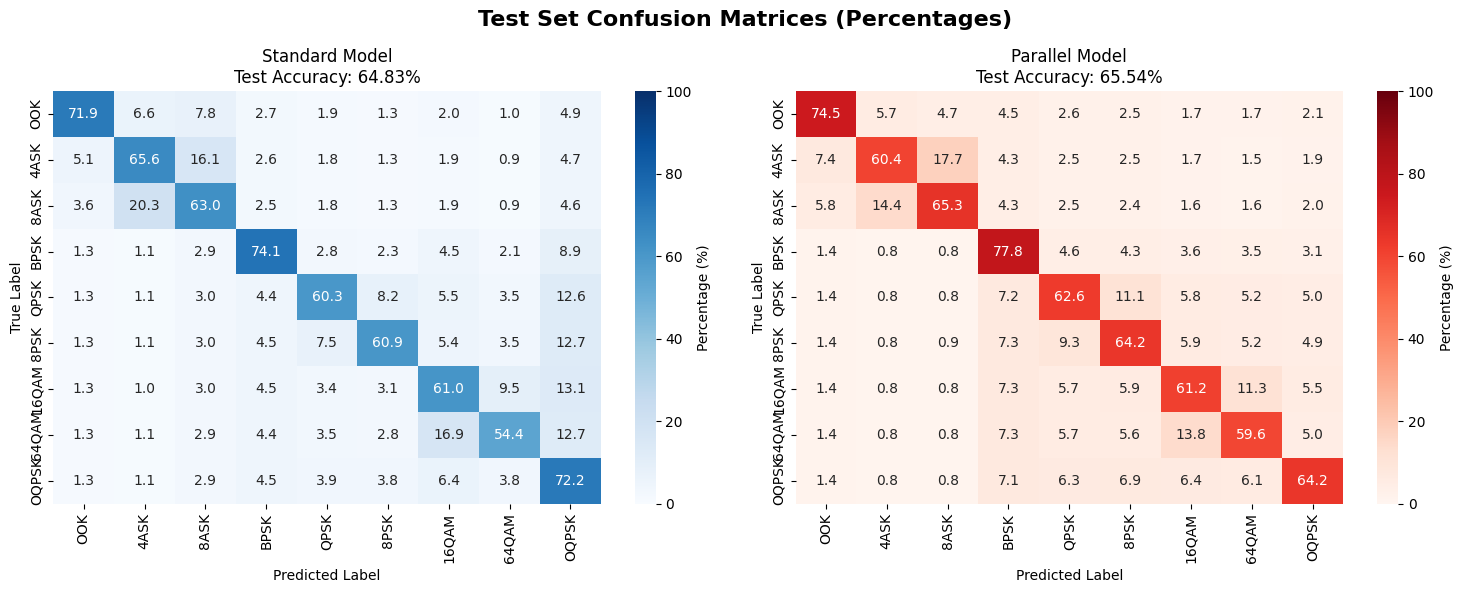
\includegraphics[width=1.0\textwidth,height=0.4\textheight]{Hasil/confusion_matrix_with_percentage.png}}
    \caption{Matriks konfusi yang membandingkan performa Model Standar (kiri) dan Model Paralel (kanan) pada set data uji. Model Paralel mencapai akurasi keseluruhan yang sedikit lebih tinggi sebesar 65,54\% dibandingkan Model Standar sebesar 64,83\%, dengan peningkatan yang signifikan pada klasifikasi modulasi 8PSK dan 64QAM.}
    \label{fig:Figure 1}
\end{figure}

Pada Figure \ref{fig:Figure 1} terlihat bahwa Model Paralel (kanan) menunjukkan peningkatan akurasi pada beberapa kelas modulasi 
dibandingkan Model Standar (kiri). Gambar tersebut yang digunakan untuk mengevaluasi kinerja dua model klasifikasi yang berbeda 
(Standar dan Paralel) dalam mengenali berbagai jenis modulasi sinyal digital (OOK, BPSK, 8PSK, dll.).

\begin{itemize}
    \item \textbf{Sumbu Vertikal (True Label):} Label atau kelas yang sebenarnya dari sinyal modulasi. 
    \item \textbf{Sumbu Horizontal (Predicted Label):} Label atau kelas yang diprediksi oleh model.
    \item \textbf{Diagonal Utama (Dari sisi Kiri atas ke Kanan Bawah):} Angka-Angka pada diagonal ini menunjukkan persentase prediksi yang benar. Semakin tinggi nilainya,
    semakin baik model tersebut dalam mengidentifiaksi kelas tersebut. Pada Model Standart (Serial), 74.1\% sinyal BPSK berhasil diidentifikasi dengan beanr sebagai BPSK
    \item \textbf{Nilai di Luar Diagonal:} Angka-angka ini menunjukkan prediksi yang salah atau "kebingungan" model. Angka ini menunjukkan kelas mana yang sering tertukar. Misalnya, pada Model Standar, 20,3\% sinyal BASK salah diklasifikasikan sebagai BPSK.
\end{itemize} 
note: \textbf{Untuk semua range SNR yang digunakan, Model Paralel menunjukkan performa yang lebih baik dibandingkan Model Standar.} 
berikut untuk analisis dan perbandingan kinerja kedua model :
\begin{itemize}
    \item \textbf{Akurasi Keseluruhan:} Model Paralel (65.54\%) lebih unggul dari pada Model Standar (64.83\%). Ini menunjukkan bahwa peningkatan performa secara umum.
    
    \item \textbf{Performa per-Kelas:}
    \begin{itemize}
        \item \textbf{Kekuatan Model Paralel:} Model paralel menunjukkan kinerja yang jauh lebih baik untuk modulasi yang lebih kompleks seperti 8PSK (64.2\% vs 60.4\%) dan 64QAM (59.6\% vs 54.4\%). Ini merupakan keunggulan utama dari model paralel yang dapat menangkap fitur-fitur kompleks dari sinyal modulasi.
        \item \textbf{Kelemahan Model Paralel:} Namun, performa Model paralel menurun untuk klasifikasi OQPSK (64.2\% vs 72.2\% pada Model Standar). Ini menunjukkan adanya trade-off antara kompleksitas model dan akurasi pada beberapa kelas modulasi.
    \end{itemize}
    
    \item \textbf{Konsistensi:} Model Paralel menunjukkan konsistensi yang lebih baik pada berbagai kelas modulasi, dengan peningkatan akurasi yang signifikan pada kelas-kelas yang lebih sulit.
    
    \item \textbf{Area Kebingungan (Di Luar Diagonal):} Kedua model menunjukkan kebingungan antara jenis modulasi yang mirip, seperti:
    \begin{itemize}
        \item Antara \textbf{QPSK} dan \textbf{OQPSK}
        \item Antara \textbf{8PSK} dan \textbf{QPSK/16QAM}
    \end{itemize}
    Ini wajar terjadi karena karakteristik sinyal mereka berdekatan.
\end{itemize}

\subsubsection{Kurva Train dan Validation ke Dua Model} 
\begin{figure}[H]
    \centerline{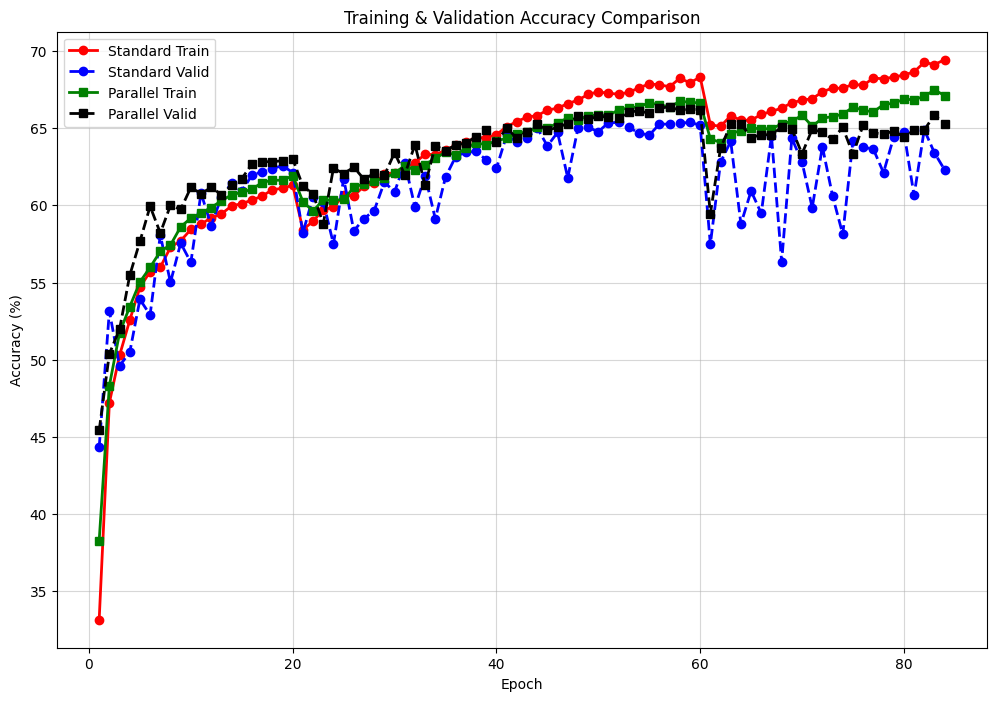
\includegraphics[width=0.9\textwidth,height=0.3\textheight]{Hasil/PRocess_Training_Validation_Accuracy.png}}
    \caption{Kurva akurasi dan loss untuk model Standar (Serial) dan Paralel pada set data pelatihan dan validasi. Model Paralel menunjukkan peningkatan akurasi yang lebih baik pada set data pelatihan dan validasi dibandingkan model Standar.}
    \label{fig:Figure 2}
\end{figure}
Pada Figure \ref{fig:Figure 2} membandingkan keinerja akurasi dari dua model, yaitu Model Standar (Serial) dan Model Paralel,
selama proses pelatihan yang diukur dalam satuan EPOCH. Kurva ini memperlihatkan bagaimana kedua model memahami dan belajar dengan 
kemampuannya untuk melakukan generalisasi terhadap data pelatihan dan validasi. Secara umum, kedua model menunjukkan proses pembelajaran yang efektif, ditandai dengan peningkatan akurasi yang signifikan pada tahap awal sebelum kurva mulai melandai. Namun, ketika membandingkan kemampuan generalisasi pada data baru, yang tercermin pada kurva validasi (garis putus-putus),
perbedaan kinerja menjadi sangat jelas. 

Kurva validasi Model Paralel (garis hitam) secara konsisten berada di posisi yang lebih tinggi dibandingkan Model Standar (garis biru), yang mengindikasikan 
bahwa Model Paralel secara superior mampu melakukan generalisasi. Lebih jauh lagi, proses pembelajaran Model Paralel terbukti jauh lebih 
stabil dan andal, terlihat dari kurvanya yang mulus. Hal ini sangat kontras dengan Model Standar yang menunjukkan fluktuasi tajam, 
termasuk penurunan drastis di sekitar epoch ke-60. Meskipun kedua model menunjukkan adanya celah antara akurasi pelatihan dan validasi—sebuah 
tanda overfitting yang wajar—kemampuan Model Paralel untuk mempertahankan akurasi validasi yang lebih tinggi dan stabil menunjukkan bahwa ia mengelola 
overfitting dengan lebih baik. Dengan demikian, dapat disimpulkan bahwa Model Paralel tidak hanya mencapai akurasi akhir yang lebih tinggi, tetapi juga menawarkan proses pembelajaran yang lebih robust, menjadikannya pilihan yang lebih unggul secara keseluruhan.

\subsubsection{Kurva Perbandingan Kerja dari Dua Model}
\begin{figure}[H]
    \centerline{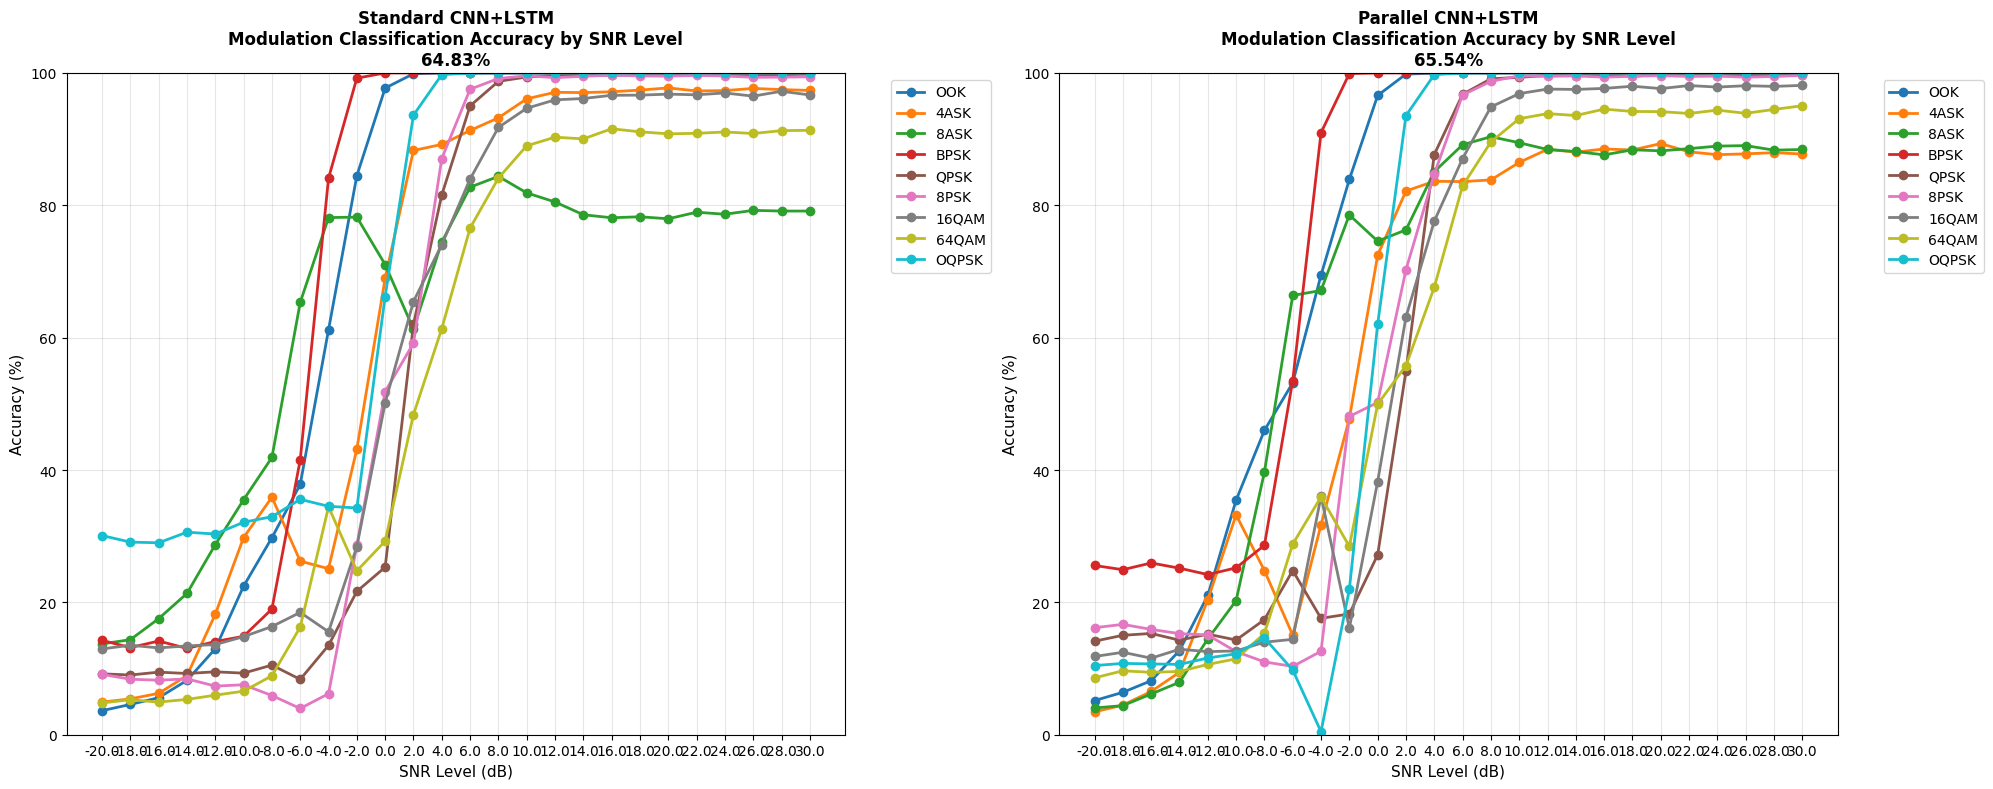
\includegraphics[width=1.2\textwidth,height=0.3\textheight]{Hasil/line_graph_overall_testing_accuracy_comparing_2model.png}}
    \caption{Kinerja klasifikasi modulasi yang menunjukkan keunggulan model Paralel (kanan) dalam mencapai akurasi tinggi pada tingkat SNR yang lebih rendah dibandingkan model Standar (kiri), terutama untuk modulasi kompleks.}
    \label{fig:Figure 3} 
\end{figure} 
Figure \ref{fig:Figure 3} menunjukkan seberapa akurat kedua model dalam menebak jenis sinyal pada berbagai tingkat kebisingan (SNR). Semakin ke kanan,
sinyal semakin jernih dan akurasi semakin tinggi untuk kedua model. Kinerja Model Paralel lebih baik daripada Model Standar.  
Model Paralel dapat mencapai tingkat akurasi yang tinggi pada rasio Signal-to-Noise (SNR) yang lebih rendah, yang merupakan 
keunggulan utamanya.  Dengan kata lain, bahkan ketika kualitas sinyal menurun secara signifikan, model ini masih dapat melakukan 
klasifikasi dengan baik. 

Selain itu, stabilitas proses pelatihan yang lebih baik mendukung model ini. Kurva Learning dari Model Paralel menunjukkan kurva validasi 
yang lebih konvergen dengan fluktuasi yang lebih kecil. Ini menunjukkan proses learning yang lebih andal. Secara kuantitatif, Model Paralel 
berkontribusi pada akurasi keseluruhan yang sedikit lebih tinggi sebesar 65,54\% dibandingkan Model Standar yang mencapai 64,83\%. Oleh karena itu 
, Model Paralel dapat dianggap sebagi arsitektur yang lebih efisien dan dapat diandalkan untuk tugas klasifikasi modulasi ini.  
\subsubsection{Heatmap Perbandingan Akurasi Per-Kelas} 
\begin{figure}[H]
    \centerline{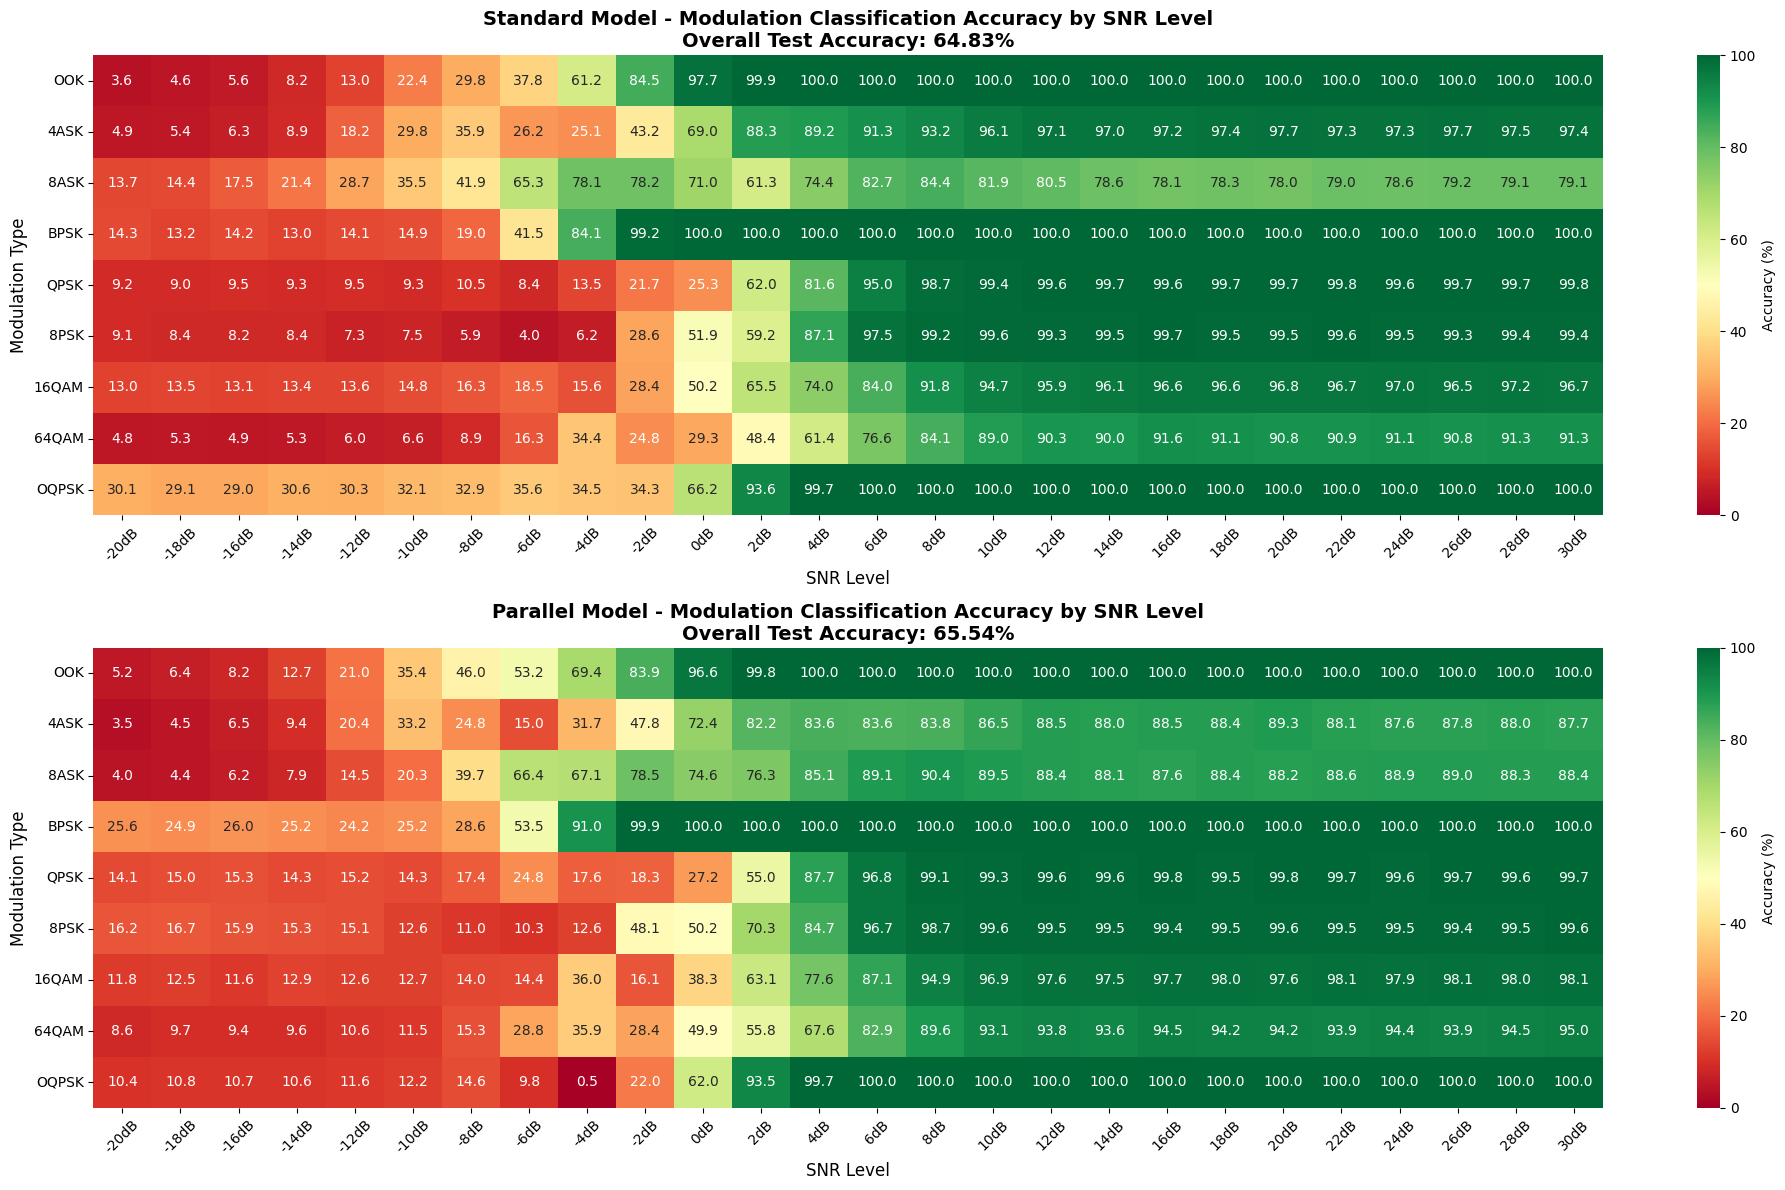
\includegraphics[width=1.0\textwidth,height=0.3\textheight]{Hasil/Heatmap_overall_testing_accuracy_comparing_2model.png}}
    \caption{Heatmap perbandingan akurasi klasifikasi antara Model Standar (atas) dan Model Paralel (bawah) untuk setiap jenis modulasi pada berbagai level SNR.}
    \label{fig:Figure 4}
\end{figure}
Figure \ref{fig:Figure 4} menyajikan perbandingan kuantitatif kinerja akurasi antara Model Standar (atas) dan Model Paralel (bawah) dalam 
bentuk heatmap. Heatmap tersebut memberikan ilustrasi secara detail performa klasifikasi untuk setiap jenis modulasi pada berbagai level SNR dari 
-20 dB hingga 30 dB. 

Secara umum, kedua model menunjukkan tren yang erwarted, di mana akurasi klasifikasi berbanding lurus dengan peningkatan level SNR. 
Hal ini terbukti dari transisi warna dari merah (akurasi rendah) ke hijau (akurasi tinggi) seiring meningkatnya kualitas sinyal. 
Namun, analisis komparatif menunjukkan keunggulan signifikan pada Model Paralel, terutama dalam hal robustisitas terhadap derau (noise).
Keunggulan ini secara visual terlihat dari transisi warna ke hijau yang terjadi pada level SNR yang lebih rendah dibandingkan dengan Model 
Standar. Sebagai contoh, pada level SNR 0 dB untuk modulasi 8PSK, Model Paralel telah mencapai akurasi sebesar 70.3\%, sementara Model Standar 
baru mencapai 51.9\%. Perbedaan efisiensi ini juga teramati pada modulasi kompleks lainnya seperti 16QAM dan 64QAM. 

Dengan demikian, analisis heatmap ini secara kuantitatif mengonfirmasi bahwa arsitektur Model Paralel lebih efektif. Kemampuannya untuk mencapai 
akurasi tinggi dalam kondisi sinyal yang lebih terdegradasi oleh derau menjadikannya pilihan yang lebih andal dan superior untuk aplikasi klasifikasi modulasi ini.


\subsection{Visualisasi Fitur dengan t-SNE} 
Untuk memahami mengapa Model Paralel menunjukkan performa yang lebih biak dibandingkan model Standar, dilakukan analsisi visualisasi fitur 
menggunakan t-Distributed Stochastic Neighbor Embedding (t-SNE). Teknik ini memvisualisasikan fitur high-dimensional yang dipelajari oleh 
kedua model dalam ruang 2D yang dapat diinterpretasikan secara visual. 

\subsubsection{\textbf{Metodologi t-SNE:}}
\begin{itemize}
    \item Ekstraksi fitur dari layer terakhir sebelum klasifikasi
    \item 2000 sampel random dari test set
    \item Parameter t-SNE: perplexity=30, max\_iter=1000
\end{itemize}

\subsubsection{\textbf{Hasil perbandingan Global}}
\begin{figure}[H]
\centerline{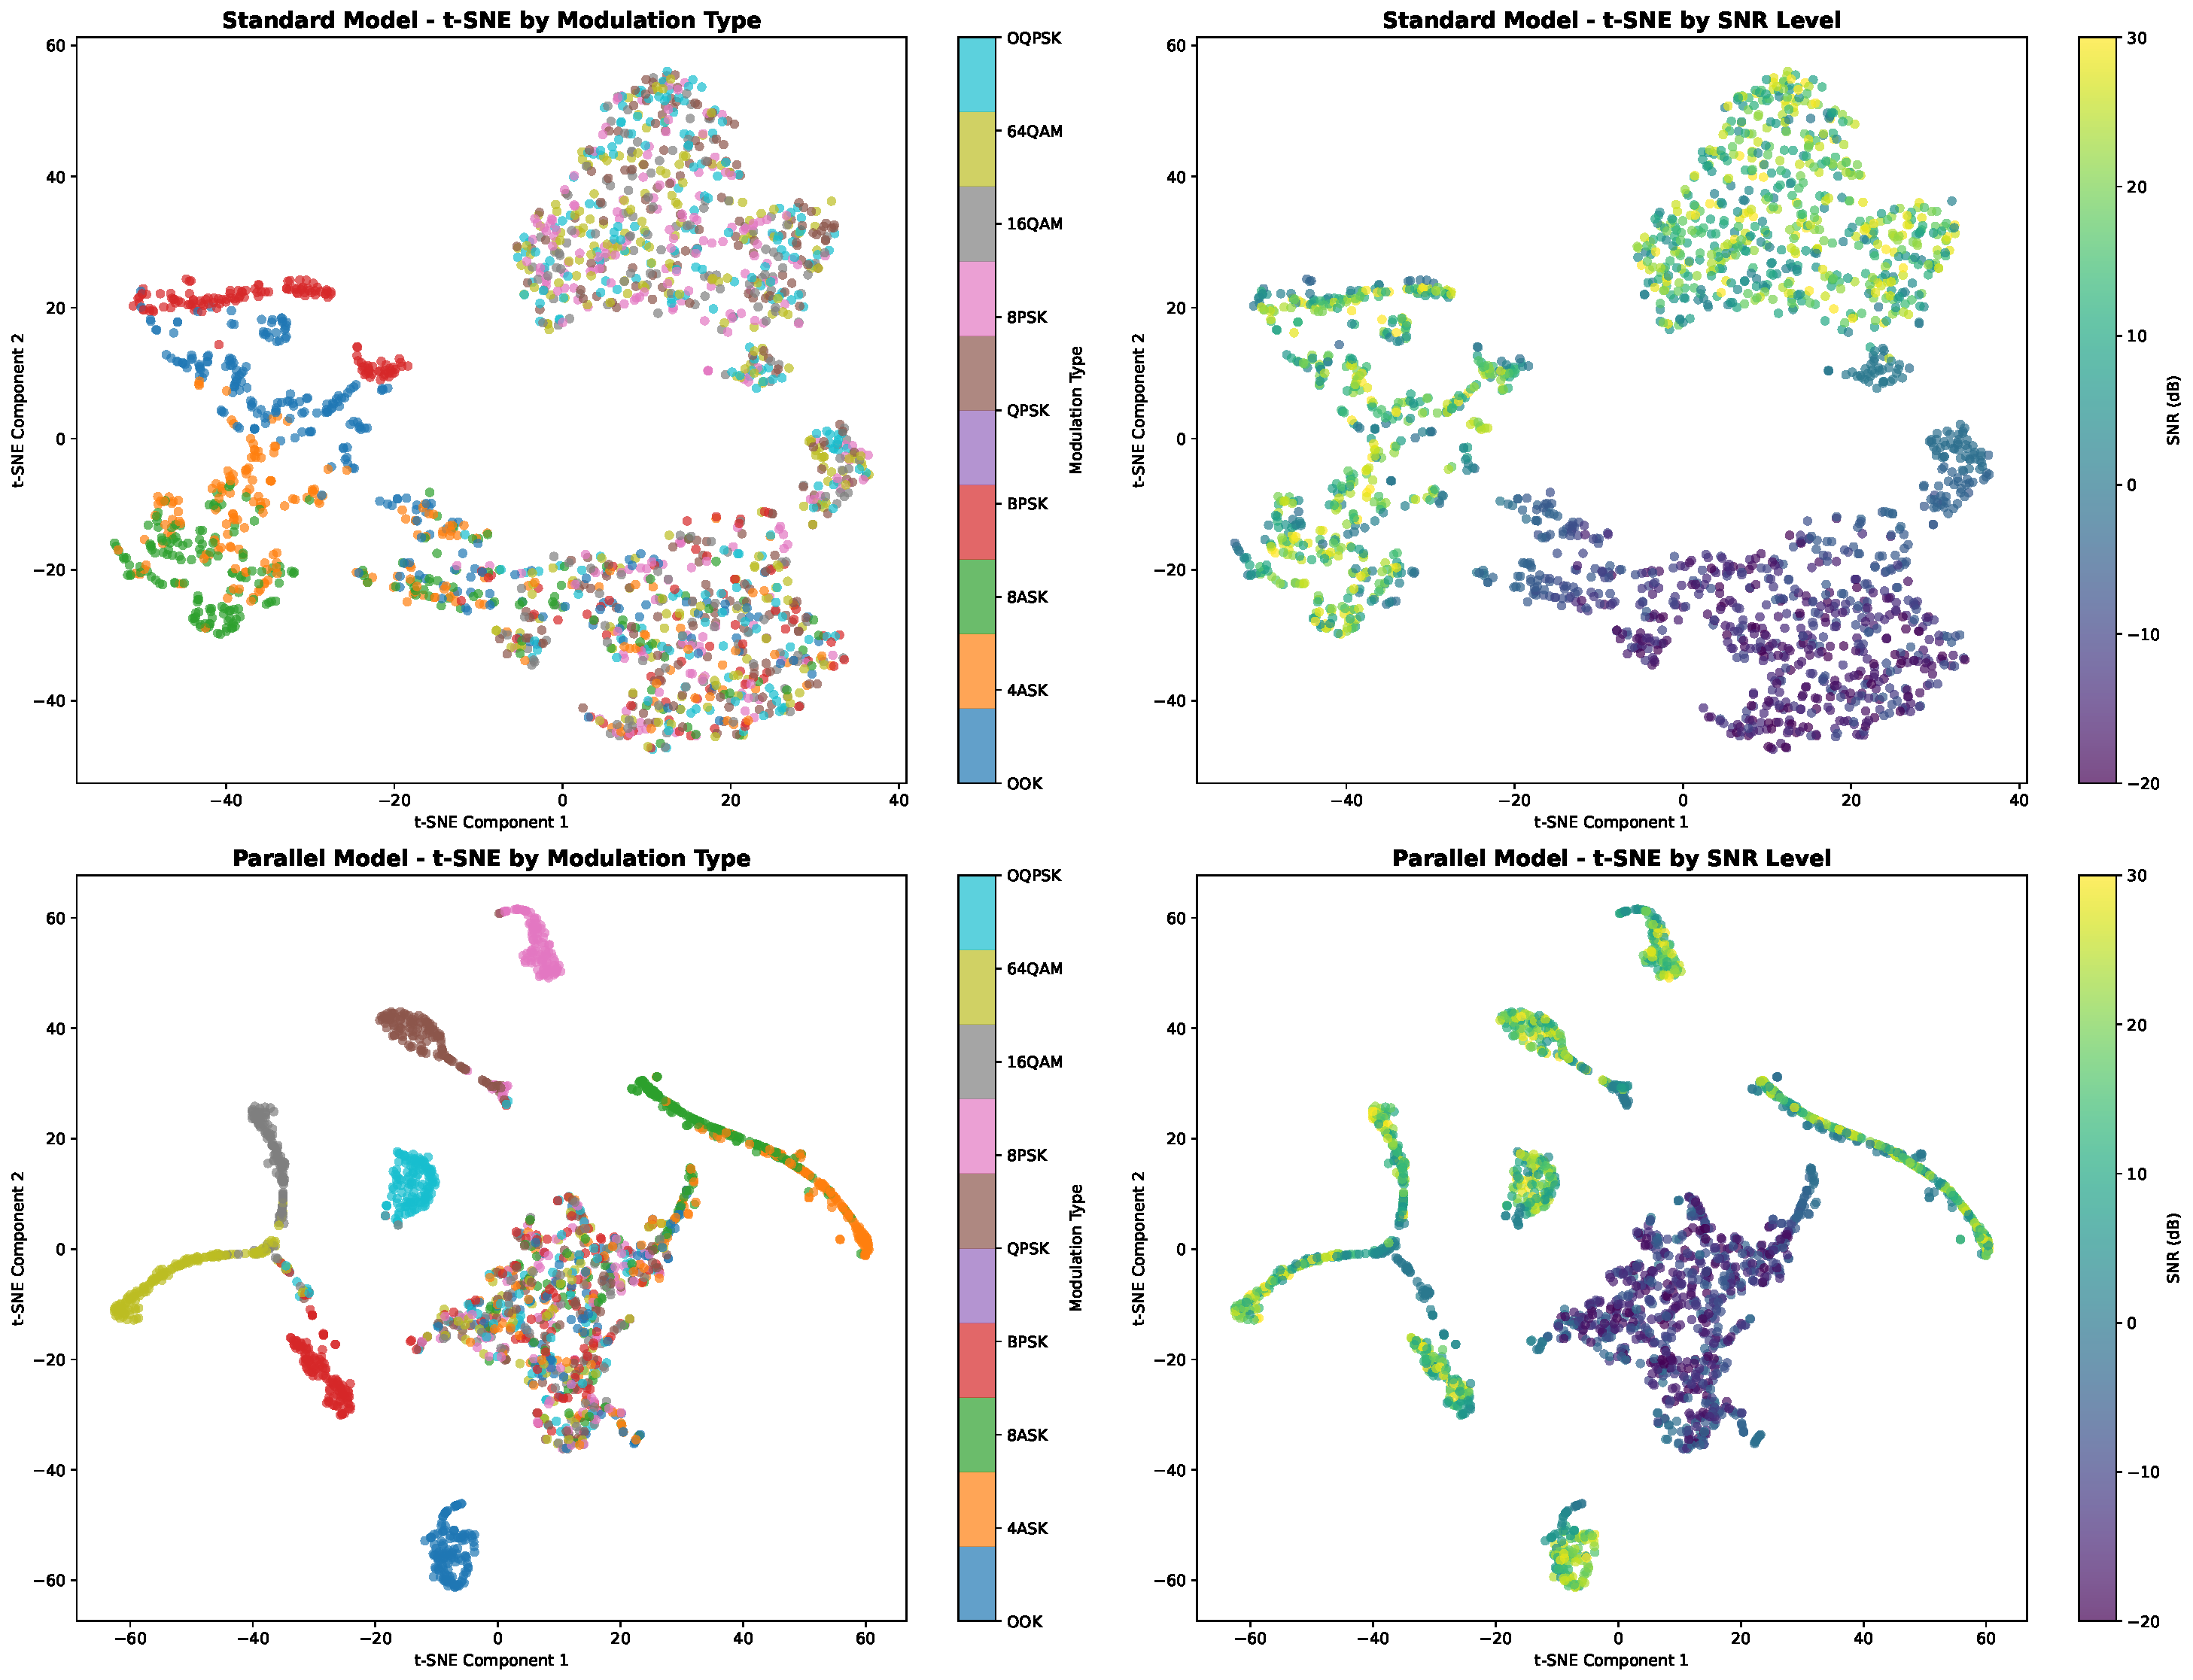
\includegraphics[width=1.0\textwidth,height=0.5\textheight]{Hasil/tsne_model_comparison.png}}
\caption{Perbandingan t-SNE antara Model Standar (atas) dan Model Paralel (bawah). Model Paralel menunjukkan clustering yang jauh lebih baik dan separasi kelas yang lebih jelas.}
\label{fig:tsne_global}
\end{figure} 
Pada Figure \ref{fig:tsne_global}, Model Paralel menghasilkan representasi fitur yang dramatically lebih terorganisir 
dibandingkan Model Standar yang menunjukkan distribusi yang scattered dan overlapping.Visualisasi t-SNE menunjukkan perbandingan 
separabilitas fitur antara Model Standar (Atas) dan Model Paralel (Bawah). Model Paralel menunjukkan clustering yang lebih jelas 
dan separasi yang lebih baik antar kelas modulasi, terutama untuk 8PSK, 16QAM, dan 64QAM

Pada Model Standar, distribusi fitur yang dihasilkan tampak kurang terstruktur. Hal ini terlihat jelas dari beberapa fenomena: 
pertama, adanya tumpang tindih (overlap) yang signifikan antara modulasi yang secara teoritis mirip, seperti QPSK dan OQPSK. 
Kedua, terjadi separasi yang buruk dan pengelompokan (clustering) yang tidak jelas untuk modulasi yang lebih kompleks, 
terutama antara 16QAM dan 64QAM. Secara keseluruhan, representasi fitur yang dipelajari oleh Model Standar tidak cukup 
diskriminatif.

Sebaliknya, Model Paralel menunjukkan superioritas yang jelas dengan menghasilkan ruang fitur yang jauh lebih terorganisir. 
Setiap kelas modulasi membentuk cluster yang lebih padat (tight) dan memiliki batas yang tegas, yang mengindikasikan bahwa model 
berhasil mempelajari fitur-fitur yang informatif. Peningkatan ini secara khusus terlihat pada separasi yang lebih baik antara 
modulasi-modulasi yang sulit dibedakan. Menurunnya tumpang tindih antar kelas dalam visualisasi ini konsisten dengan hasil kuantitatif 
yang ditunjukkan pada confusion matrix, yang mengonfirmasi bahwa arsitektur paralel secara fundamental lebih efektif dalam tugas klasifikasi ini.
\newpage 

\subsubsection{\textbf{Hasil Perbadingan Per-Kelas}}
\begin{figure}[H]
\centerline{
\includegraphics[width=1.0\textwidth]{Hasil/tsne_detailed_analysis.png}}
\caption{Analisis t-SNE per-kelas menunjukkan setiap jenis modulasi. Model Paralel (bawah) menghasilkan struktur yang organized untuk semua kelas, sementara Model Standar (atas) menunjukkan distribusi yang chaotic.}
\label{fig:tsne_per_class}
\end{figure}
Figure \ref{fig:tsne_per_class} menyajikan visualisasi t-SNE yang digunakan untuk menganalisis ruang fitur (\textit{feature space}) yang dipelajari oleh kedua model. 
Visualisasi ini memetakan fitur-fitur yang diekstraksi dari \textit{layer} terakhir sebelum klasifikasi ke dalam ruang 2D untuk mengamati kemampuan separasi kelas dari masing-masing model.

Pada \textbf{Model Standar} (baris atas), terlihat bahwa fitur-fitur untuk setiap kelas modulasi cenderung tersebar dan tumpang tindih secara signifikan dengan fitur dari kelas lain (direpresentasikan oleh titik abu-abu). 
Hal ini mengindikasikan bahwa model tersebut kesulitan membentuk batas keputusan yang jelas antar kelas, sehingga menghasilkan representasi fitur yang kurang diskriminatif.

Sebaliknya, \textbf{Model Paralel} (baris bawah) menunjukkan hasil yang jauh lebih superior. Fitur untuk setiap kelas membentuk \textit{cluster} atau manifold yang padat, terstruktur, dan memiliki separasi yang jelas dari kelas lainnya. 
Lebih lanjut, di dalam setiap \textit{cluster}, teramati adanya gradasi warna yang mulus sesuai dengan level SNR, dari ungu (SNR rendah) ke kuning (SNR tinggi). 
Fenomena ini membuktikan bahwa Model Paralel tidak hanya mampu mempelajari fitur yang sangat diskriminatif untuk memisahkan kelas, tetapi juga berhasil menangkap struktur internal data yang berkorelasi dengan kualitas sinyal. 
Dengan demikian, analisis t-SNE ini secara kualitatif mengonfirmasi bahwa Model Paralel memiliki kemampuan representasi fitur yang jauh lebih efektif dan teratur dibandingkan Model Standar.


\end{document}
